%%mark = star, diamond, square, otimes
%\documentclass{article}
%\usepackage{pgfplots}
%\usepackage[justification=centering]{caption}
%\pgfplotsset{compat=newest}
%\begin{document}
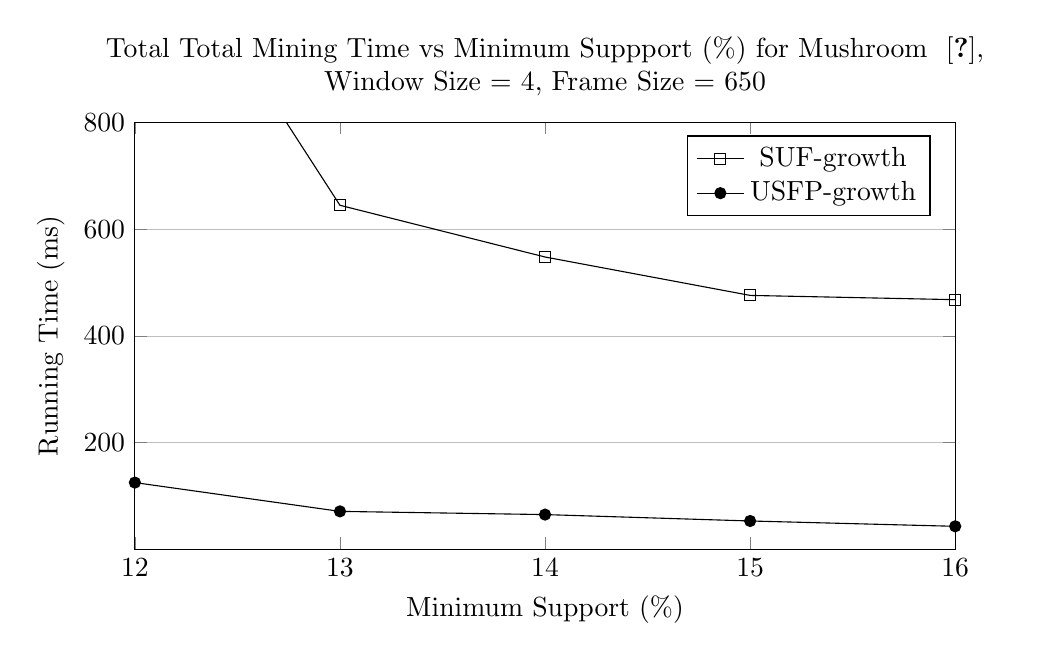
\begin{tikzpicture}
\begin{axis}[
	title={\parbox{\linewidth}{\centering Total Total Mining Time vs Minimum Suppport (\%) for Mushroom ~\cite{dataset}, Window Size = 4, Frame Size = 650}},
	width=12cm,
	height=7cm,
    xlabel={Minimum Support (\%) },
    ylabel={Running Time (ms)},
    xmin=12, xmax=16,
    ymin=0, ymax=800,
    xtick={12,13,14,15,16},
    ytick={200,400,600,800},
    legend pos=north east,
    ymajorgrids=true,
    grid style={line width=.2pt,draw=gray!50},
]
 
\addplot[
    solid, every mark/.append style={solid, fill=gray}, mark=square
    ]
    coordinates {
	(12,1240)
	(13,645)
	(14,548)
	(15,476)
	(16,468)

};
    \addlegendentry{SUF-growth}
\addplot[
    solid, every mark/.append style={solid, fill=black}, mark=*
    ]
    coordinates {
	(12,125)
	(13,71 )
	(14,65 )
	(15,53 )
	(16,43 )

};
    \addlegendentry{USFP-growth}
 
\end{axis}
\end{tikzpicture}
%\end{document}